
\chapter{Glosario, acrónimos y abreviaturas}

Este anexo reúne, en primer lugar, las definiciones de los términos de dominio
empleados a lo largo de la memoria y, en segundo lugar, la expansión de las
siglas y abreviaturas utilizadas. Su finalidad es facilitar una lectura
autocontenida del documento, evitando que el lector deba recurrir a la sección
en la que cada concepto se introduce por primera vez.

\section{Glosario}

\begin{description}
	\item[Alucinación] Fenómeno por el cual un modelo de lenguaje genera información
	      inexistente o no respaldada por las tripletas de entrada. Es una de las
	      limitaciones que el proceso de validación y revisión trata de contener.
	\item[Anotación] Sentencia en español redactada para verbalizar el contenido de una
	      entrada. En la aplicación se persiste por frase y queda asociada a su autor.
	\item[Anotador] Usuario encargado de transformar las tripletas RDF en texto en
	      lenguaje natural y de corregir las traducciones automáticas.
	\item[\textit{Benchmark}] Conjunto de datos y protocolo de evaluación estandarizado
	      que permite entrenar, comparar y clasificar sistemas bajo condiciones
	      homogéneas.
	\item[Cobertura] Grado en que una verbalización refleja todos los hechos contenidos
	      en el conjunto de tripletas que describe.
	\item[Corpus] Colección estructurada de textos ---en este trabajo, alineados con
	      conjuntos de tripletas RDF--- empleada para entrenar y evaluar modelos.
	\item[\textit{Crowdsourcing}] Estrategia de producción de datos basada en la
	      colaboración distribuida de múltiples participantes; sustenta el reparto del
	      trabajo de anotación y revisión.
	\item[\textit{Dataset} (conjunto de datos)] Unidad principal de trabajo de la
	      plataforma: un corpus importado, con sus entradas, su configuración y su estado
	      de progreso.
	\item[DBpedia] Base de conocimiento multilingüe extraída de Wikipedia y publicada
	      como tripletas RDF; es la fuente de las tripletas de WebNLG.
	\item[Diversidad] Criterio de revisión, evaluado una sola vez por entrada, que valora
	      la variedad lingüística entre las distintas frases de una misma entrada.
	\item[\textit{Embedding}] Representación vectorial de una palabra o un texto en un
	      espacio continuo, utilizada por métricas semánticas como BERTScore.
	\item[Entrada (\textit{entry})] Elemento del corpus formado por un conjunto de
	      tripletas y sus verbalizaciones asociadas, junto con sus metadatos (categoría,
	      forma, tamaño y estado).
	\item[Evento n-ario] Construcción que relaciona varios participantes o atributos en
	      torno a un mismo hecho, equivalente a una agregación en el modelado de datos, y
	      que no puede representarse con una única tripleta binaria sin pérdida de
	      información.
	\item[Lexicalización (\textit{lex})] Verbalización en lenguaje natural de una entrada
	      en un idioma determinado.
	\item[\textit{Linked Open Data}] Iniciativa de publicación de datos enlazados y
	      abiertos en la web mediante RDF, de la que DBpedia es uno de los nodos
	      centrales.
	\item[Moderador] Rol de servidor elevado, con capacidad para crear \textit{datasets},
	      acceder a la API de administración y gestionar criterios.
	\item[Permiso (\textit{permit})] Conjunto de capacidades de un usuario sobre un
	      \textit{dataset} concreto: propiedad, anotación, revisión y administración.
	\item[Predicado] Componente central de una tripleta RDF que expresa la propiedad o
	      relación que vincula al sujeto con el objeto.
	\item[Revisión] Segunda capa de aseguramiento de la calidad en la que un revisor
	      valida las anotaciones conforme a un conjunto de criterios.
	\item[Revisor] Usuario encargado de evaluar las anotaciones de otros participantes;
	      no puede revisar sus propias anotaciones.
	\item[Sección] Bloque de entradas que constituye la unidad de trabajo asignable a un
	      usuario, de modo que la sesión de anotación resulte manejable.
	\item[\textit{Semantic parsing}] Tarea inversa a la generación: obtención de una
	      estructura RDF a partir de un texto en lenguaje natural.
	\item[Sujeto] Componente de una tripleta RDF que identifica la entidad descrita.
	\item[Objeto] Componente de una tripleta RDF que aporta el valor de la propiedad o la
	      entidad relacionada con el sujeto.
	\item[Tripleta (RDF)] Hecho atómico de la forma \emph{(sujeto, predicado, objeto)},
	      en el que cada componente se identifica mediante una URI.
	\item[\textit{Tripleset}] Conjunto de tripletas asociado a una entrada. Puede ser de
	      tipo \texttt{original} o \texttt{modified}.
	\item[Verbalización] Expresión en lenguaje natural del contenido de un conjunto de
	      tripletas.
	\item[WebNLG] \textit{Dataset} y \textit{benchmark} que relaciona conjuntos de
	      tripletas RDF de DBpedia con verbalizaciones de su contenido en lenguaje
	      natural.
\end{description}

\section{Acrónimos y abreviaturas}

\begin{longtable}{|p{0.16\linewidth}|p{0.76\linewidth}|}
	\hline
	\textbf{Sigla} & \textbf{Significado}                                                                          \\
	\hline
	\endhead
	API            & \textit{Application Programming Interface} (interfaz de programación de aplicaciones).        \\ \hline
	BENG           & \textit{Benchmarking Environment for NLG}; plataforma de evaluación empleada en WebNLG+ 2020. \\ \hline
	BERT           & \textit{Bidirectional Encoder Representations from Transformers}.                             \\ \hline
	BLEU           & \textit{Bilingual Evaluation Understudy}; métrica de evaluación de generación.                \\ \hline
	B2 / C1        & Niveles de competencia lingüística del MCER.                                                  \\ \hline
	chrF / chrF++  & \textit{Character n-gram F-score} y su extensión con \textit{n-gramas} de palabra.            \\ \hline
	COMET          & \textit{Crosslingual Optimized Metric for Evaluation of Translation}.                         \\ \hline
	CSS            & \textit{Cascading Style Sheets}.                                                              \\ \hline
	\texttt{dbo:}  & \textit{DBpedia Ontology}; espacio de nombres de clases y propiedades de DBpedia.             \\ \hline
	\texttt{dbr:}  & \textit{DBpedia Resource}; espacio de nombres de los recursos de DBpedia.                     \\ \hline
	DOM            & \textit{Document Object Model}.                                                               \\ \hline
	DTO            & \textit{Data Transfer Object} (objeto de transferencia de datos).                             \\ \hline
	ETSIINF        & Escuela Técnica Superior de Ingenieros Informáticos (UPM).                                    \\ \hline
	GERBIL         & \textit{General Entity Annotator Benchmarking Framework}; plataforma de evaluación.           \\ \hline
	HTTP           & \textit{Hypertext Transfer Protocol}.                                                         \\ \hline
	IA             & Inteligencia Artificial.                                                                      \\ \hline
	JSON           & \textit{JavaScript Object Notation}.                                                          \\ \hline
	LLM            & \textit{Large Language Model} (gran modelo de lenguaje).                                      \\ \hline
	MCER           & Marco Común Europeo de Referencia para las lenguas.                                           \\ \hline
	METEOR         & \textit{Metric for Evaluation of Translation with Explicit ORdering}.                         \\ \hline
	NLG            & \textit{Natural Language Generation} (generación de lenguaje natural).                        \\ \hline
	NLP / PLN      & \textit{Natural Language Processing} / Procesamiento del Lenguaje Natural.                    \\ \hline
	ORM            & \textit{Object-Relational Mapping} (mapeo objeto-relacional).                                 \\ \hline
	RDF            & \textit{Resource Description Framework}.                                                      \\ \hline
	SGBD           & Sistema Gestor de Bases de Datos.                                                             \\ \hline
	SPARQL         & \textit{SPARQL Protocol and RDF Query Language}.                                              \\ \hline
	SQL            & \textit{Structured Query Language}.                                                           \\ \hline
	TER            & \textit{Translation Edit Rate}.                                                               \\ \hline
	TFM            & Trabajo de Fin de Máster.                                                                     \\ \hline
	UPM            & Universidad Politécnica de Madrid.                                                            \\ \hline
	URI            & \textit{Uniform Resource Identifier}.                                                         \\ \hline
	URL            & \textit{Uniform Resource Locator}.                                                            \\ \hline
	WebNLG         & \textit{Web Natural Language Generation}.                                                     \\ \hline
	XML            & \textit{eXtensible Markup Language}.                                                          \\ \hline
	XSD            & \textit{XML Schema Definition}.                                                               \\ \hline
\end{longtable}

\chapter{Esquema entidad-relación}

Este anexo describe el modelo de datos relacional sobre el que se asienta la
aplicación \texttt{lanbench}. La fuente única de verdad del modelo es el
esquema declarativo \texttt{prisma/schema.prisma}, que se materializa en
MariaDB mediante la operación \texttt{prisma db push}. Una representación
gráfica equivalente puede obtenerse en cualquier momento desde Prisma Studio o
desde el explorador Adminer descritos en el capítulo de la aplicación.

\section{Visión general}

El esquema está normalizado y se organiza en torno a dos agregados principales:
el \textbf{dataset}, que gobierna la organización del trabajo y los permisos, y
la \textbf{entrada} (\textit{entry}), que concentra el contenido RDF y todo lo
que se deriva de él (verbalizaciones, anotaciones y revisiones). El resto de
tablas dan soporte al control de acceso, a la asistencia mediante IA y a la
operación del servidor. La Figura~\ref{fig:er-modelo} ofrece la representación
gráfica del esquema.

\begin{landscape}
	\begin{figure}[H]
		\centering
		\resizebox{0.98\linewidth}{!}{%
			\begin{tikzpicture}[
					font=\sffamily\scriptsize,
					entity/.style={
							rectangle,
							draw=black,
							fill=gray97,
							minimum width=3.1cm,
							minimum height=0.72cm,
							align=center
						},
					core/.style={
							rectangle,
							draw=black,
							fill=gray75,
							minimum width=3.3cm,
							minimum height=0.78cm,
							align=center,
							font=\sffamily\scriptsize\bfseries
						},
					assoc/.style={
							rectangle,
							draw=black,
							fill=white,
							minimum width=3.1cm,
							minimum height=0.72cm,
							align=center
						},
					independent/.style={
							rectangle,
							draw=black,
							dashed,
							fill=white,
							minimum width=3.1cm,
							minimum height=0.72cm,
							align=center
						},
					rel/.style={-{Latex[length=2.0mm]}, thick},
					logical/.style={-{Latex[length=1.8mm]}, dashed},
					card/.style={font=\sffamily\tiny, fill=white, inner sep=1pt}
				]
				\node[core] (dataset) at (0, 0) {Dataset\\\texttt{datasets}};
				\node[core] (entry) at (0, -3.0) {Entry\\\texttt{entries}};

				\node[entity] (section) at (-5.2, 1.4) {Section\\\texttt{sections}};
				\node[assoc] (permit) at (-5.2, 0.0) {Permit\\\texttt{permits}};
				\node[entity] (credential) at (-5.2, -1.4) {DatasetLlmCredential\\\texttt{dataset\_llm\_credentials}};
				\node[entity] (assignment) at (-5.2, -2.8) {SectionAssignment\\\texttt{section\_assignments}};
				\node[entity] (active) at (-5.2, -4.2) {ActiveSession\\\texttt{active\_sessions}};
				\node[core] (user) at (-10.2, -3.2) {User\\\texttt{users}};

				\node[entity] (tripleset) at (5.0, -1.2) {Tripleset\\\texttt{triplesets}};
				\node[entity] (triple) at (9.4, -1.2) {Triple\\\texttt{triples}};
				\node[entity] (lex) at (5.0, -2.4) {Lex\\\texttt{lexes}};
				\node[entity] (link) at (5.0, -3.6) {Link\\\texttt{links}};
				\node[entity] (dbpedia) at (5.0, -4.8) {DbpediaLink\\\texttt{dbpedia\_links}};

				\node[entity] (annotation) at (-0.3, -6.6) {Annotation\\\texttt{annotations}};
				\node[entity] (alert) at (-5.2, -6.6) {AnnotationAlertDecision\\\texttt{annotation\_alert\_decisions}};
				\node[entity] (review) at (4.8, -6.6) {Review\\\texttt{reviews}};
				\node[entity] (decision) at (9.4, -5.8) {ReviewDecision\\\texttt{review\_decisions}};
				\node[entity] (comment) at (9.4, -7.4) {ReviewComment\\\texttt{review\_comments}};
				\node[independent] (criterion) at (13.2, -6.6) {EvaluationCriterion\\\texttt{evaluation\_criteria}};

				\node[independent] (register) at (-10.2, 1.2) {RegisterCode\\\texttt{register\_codes}};
				\node[independent] (session) at (-10.2, 0.0) {Session\\\texttt{sessions}};

				\draw[rel] (dataset) -- node[card, above] {1:N} (section);
				\draw[rel] (dataset) -- node[card, above] {1:N} (permit);
				\draw[rel] (dataset) -- node[card, above] {1:N} (credential);
				\draw[rel] (dataset) -- node[card, above] {1:N} (assignment);
				\draw[rel] (dataset) -- node[card, above] {1:N} (active);
				\draw[rel] (dataset) -- node[card, right] {1:N} (entry);

				\draw[rel] (user) -- node[card, above] {1:N} (permit);
				\draw[rel] (user) -- node[card, above] {1:N} (assignment);
				\draw[rel] (user) -- node[card, below] {1:N} (active);
				\draw[logical] (user) to[bend left=24] node[card, below, pos=0.34] {N:M vía Permit} (dataset);

				\draw[rel] (entry) -- node[card, above] {1:N} (tripleset);
				\draw[rel] (tripleset) -- node[card, above] {1:N} (triple);
				\draw[rel] (entry) -- node[card, above] {1:N} (lex);
				\draw[rel] (entry) -- node[card, above] {1:N} (link);
				\draw[rel] (entry) -- node[card, above] {1:N} (dbpedia);

				\draw[rel] (entry) -- node[card, left] {1:N} (annotation);
				\draw[rel] (entry) -- node[card, above] {1:N} (alert);
				\draw[rel] (entry) -- node[card, right] {1:N} (review);
				\draw[rel] (user) to[out=-35, in=180] node[card, near end, above] {1:N} (alert);
				\draw[rel] (user.south) -- ++(0, -4.25) -| node[card, pos=0.24, below] {1:N} (annotation.south);
				\draw[rel] (user.south) -- ++(0, -4.75) -| node[card, pos=0.24, below] {1:N revisor/anotador} (review.south);

				\draw[rel] (review) -- node[card, above] {1:N} (decision);
				\draw[rel] (review) -- node[card, below] {1:N} (comment);
				\draw[logical] (criterion) to[out=150, in=0] node[card, above] {código lógico} (decision);
			\end{tikzpicture}%
		}
		\caption{Diagrama entidad-relación del esquema de datos de
			\texttt{lanbench}.}
		\label{fig:er-modelo}
	\end{figure}
\end{landscape}

La jerarquía de composición principal, leída de arriba abajo, es la siguiente:

\begin{itemize}
	\item \textbf{Dataset} \(\rightarrow\) Secciones, Permisos, Asignaciones de sección,
	      Sesiones activas, Credenciales de IA.
	\item \textbf{Dataset} \(\rightarrow\) \textbf{Entrada} \(\rightarrow\)
	      \begin{itemize}
		      \item \textit{Triplesets} \(\rightarrow\) Tripletas.
		      \item Lexicalizaciones, Enlaces y Enlaces DBpedia.
		      \item Anotaciones y Decisiones sobre alertas.
		      \item \textbf{Revisiones} \(\rightarrow\) Decisiones de revisión y Comentarios de
		            revisión.
	      \end{itemize}
\end{itemize}

\section{Entidades}

La siguiente tabla inventaría las entidades del modelo, agrupadas por área
funcional, con su nombre de modelo, su tabla física y una descripción breve.

\begin{longtable}{|p{0.22\linewidth}|p{0.24\linewidth}|p{0.42\linewidth}|}
	\hline
	\textbf{Modelo}         & \textbf{Tabla}                        & \textbf{Descripción}                                                                                  \\
	\hline
	\endhead
	\multicolumn{3}{|l|}{\textit{Usuarios y control de acceso}}                                                                                                             \\ \hline
	User                    & \texttt{users}                        & Usuario del sistema; correo único, contraseña e indicador de moderador.                               \\ \hline
	Permit                  & \texttt{permits}                      & Capacidades de un usuario sobre un \textit{dataset} (propiedad, anotación, revisión, administración). \\ \hline
	RegisterCode            & \texttt{register\_codes}              & Códigos de un solo uso para el registro directo de moderadores.                                       \\ \hline
	Session                 & \texttt{sessions}                     & Sesiones de \texttt{express-session} persistidas en base de datos.                                    \\ \hline
	\multicolumn{3}{|l|}{\textit{Datasets y organización del trabajo}}                                                                                                      \\ \hline
	Dataset                 & \texttt{datasets}                     & Corpus importado; metadatos, modo de LLM, opciones de revisión y contadores de progreso.              \\ \hline
	Section                 & \texttt{sections}                     & Asociación de cada sección de un \textit{dataset} con su bloque.                                      \\ \hline
	SectionAssignment       & \texttt{section\_assignments}         & Reserva temporal de una sección a un usuario, con caducidad y tiempo dedicado.                        \\ \hline
	ActiveSession           & \texttt{active\_sessions}             & Posición de trabajo en curso (sección y entrada) por usuario, \textit{dataset} y modo.                \\ \hline
	DatasetLlmCredential    & \texttt{dataset\_llm\_credentials}    & Credenciales de proveedor de IA por \textit{dataset}, con la clave cifrada.                           \\ \hline
	\multicolumn{3}{|l|}{\textit{Contenido RDF}}                                                                                                                            \\ \hline
	Entry                   & \texttt{entries}                      & Entrada del corpus: categoría, forma, tamaño, posición y estado.                                      \\ \hline
	Tripleset               & \texttt{triplesets}                   & Conjunto de tripletas de una entrada, de tipo \texttt{original} o \texttt{modified}.                  \\ \hline
	Triple                  & \texttt{triples}                      & Tripleta sujeto--predicado--objeto.                                                                   \\ \hline
	Lex                     & \texttt{lexes}                        & Lexicalización (verbalización) de una entrada en un idioma.                                           \\ \hline
	Link                    & \texttt{links}                        & Enlaces semánticos asociados a la entrada.                                                            \\ \hline
	DbpediaLink             & \texttt{dbpedia\_links}               & Enlaces a DBpedia asociados a la entrada.                                                             \\ \hline
	\multicolumn{3}{|l|}{\textit{Anotación}}                                                                                                                                \\ \hline
	Annotation              & \texttt{annotations}                  & Sentencia en español de una frase de una entrada, con su origen y estado.                             \\ \hline
	AnnotationAlertDecision & \texttt{annotation\_alert\_decisions} & Decisión del anotador sobre cada alerta automática (aceptación u omisión justificada).                \\ \hline
	\multicolumn{3}{|l|}{\textit{Revisión}}                                                                                                                                 \\ \hline
	EvaluationCriterion     & \texttt{evaluation\_criteria}         & Catálogo de criterios de calidad, ordenados y versionados.                                            \\ \hline
	Review                  & \texttt{reviews}                      & Revisión de una entrada por un revisor sobre las anotaciones de un anotador.                          \\ \hline
	ReviewDecision          & \texttt{review\_decisions}            & Decisión binaria por criterio (y frase) dentro de una revisión.                                       \\ \hline
	ReviewComment           & \texttt{review\_comments}             & Corrección textual aportada durante la revisión.                                                      \\ \hline
\end{longtable}

\section{Relaciones}

La tabla siguiente recoge las relaciones entre entidades con su cardinalidad.
Salvo indicación en contra, se trata de relaciones uno a varios (1:N)
materializadas mediante clave ajena.

\begin{longtable}{|p{0.40\linewidth}|p{0.13\linewidth}|p{0.35\linewidth}|}
	\hline
	\textbf{Relación}                       & \textbf{Card.} & \textbf{Descripción}                                                                        \\
	\hline
	\endhead
	Dataset -- Section                      & 1:N            & Un \textit{dataset} se divide en secciones.                                                 \\ \hline
	Dataset -- Entry                        & 1:N            & Un \textit{dataset} contiene múltiples entradas.                                            \\ \hline
	User -- Dataset (vía Permit)            & N:M            & Relación de permisos con atributos de rol; clave primaria compuesta.                        \\ \hline
	Dataset / User -- SectionAssignment     & 1:N            & Reserva de secciones a usuarios.                                                            \\ \hline
	Dataset / User -- ActiveSession         & 1:N            & Sesión de trabajo activa por \textit{dataset}, usuario y modo.                              \\ \hline
	Dataset -- DatasetLlmCredential         & 1:N            & Credenciales de IA por proveedor (única por \textit{dataset} y proveedor).                  \\ \hline
	Entry -- Tripleset                      & 1:N            & Conjuntos de tripletas de una entrada.                                                      \\ \hline
	Tripleset -- Triple                     & 1:N            & Tripletas que componen un \textit{tripleset}.                                               \\ \hline
	Entry -- Lex                            & 1:N            & Lexicalizaciones de la entrada.                                                             \\ \hline
	Entry -- Link                           & 1:N            & Enlaces semánticos de la entrada.                                                           \\ \hline
	Entry -- DbpediaLink                    & 1:N            & Enlaces a DBpedia de la entrada.                                                            \\ \hline
	Entry / User -- Annotation              & 1:N            & Anotaciones de una entrada; clave primaria compuesta por entrada, \textit{dataset} y frase. \\ \hline
	Entry / User -- AnnotationAlertDecision & 1:N            & Decisiones sobre alertas automáticas.                                                       \\ \hline
	Entry -- Review                         & 1:N            & Revisiones de una entrada.                                                                  \\ \hline
	User -- Review (revisor)                & 1:N            & Revisiones realizadas como revisor.                                                         \\ \hline
	User -- Review (anotador)               & 1:N            & Revisiones recibidas como anotador.                                                         \\ \hline
	Review -- ReviewDecision                & 1:N            & Decisiones por criterio dentro de la revisión.                                              \\ \hline
	Review -- ReviewComment                 & 1:N            & Comentarios y correcciones de la revisión.                                                  \\ \hline
\end{longtable}

\section{Notas de diseño}

\begin{itemize}
	\item \textbf{Claves primarias compuestas}: \texttt{permits} (\texttt{dataset\_id},
	      \texttt{user\_id}), \texttt{annotations} (\texttt{entry\_id},
	      \texttt{dataset\_id}, \texttt{sentence\_index}) y \texttt{active\_sessions}
	      (\texttt{dataset\_id}, \texttt{user\_id}, \texttt{mode}).
	\item \textbf{Enumerado}: el tipo de \textit{tripleset} se restringe al enumerado
	      \texttt{TriplesetType}, con los valores \texttt{original} y \texttt{modified}.
	\item \textbf{Reglas de borrado}: el contenido derivado de una entrada o de un
	      \textit{dataset} se elimina en cascada; en cambio, \texttt{permits} y
	      \texttt{sections} aplican \texttt{Restrict} para proteger la integridad
	      referencial, y las credenciales de IA se eliminan en cascada con su
	      \textit{dataset}.
	\item \textbf{Unicidad del criterio de diversidad}: en \texttt{review\_decisions}, la
	      diversidad es un criterio a nivel de entrada y su \texttt{sentence\_index} es
	      \texttt{NULL}. Dado que MariaDB trata los valores nulos como distintos en los
	      índices únicos, su unicidad se garantiza en el repositorio (mediante
	      \textit{find-then-upsert}) y no por la restricción de base de datos.
	\item \textbf{Tablas independientes}: \texttt{evaluation\_criteria},
	      \texttt{register\_codes} y \texttt{sessions} no participan en relaciones de
	      clave ajena; las dos últimas dan soporte, respectivamente, al registro de
	      moderadores y a la persistencia de sesiones.
\end{itemize}

\chapter{Manual de usuario}

Este anexo describe, paso a paso, el uso de la aplicación \texttt{lanbench}
desde la perspectiva de cada rol. Se asume que la plataforma se encuentra ya
desplegada y accesible ---en el entorno de desarrollo, en
\texttt{http://localhost:3000}--- y que el usuario dispone de un navegador web.

\section{Acceso a la plataforma}

\subsection{Registro}

Desde la página de registro (\texttt{/register}) el visitante introduce su
correo electrónico, su nombre y apellidos y una contraseña, que debe repetir
para confirmarla. Quien disponga de un \textbf{código de moderador} ---una cadena
de exactamente dieciséis caracteres alfanuméricos y de un solo uso--- puede
indicarlo en el campo correspondiente para registrarse directamente con
privilegios elevados, sin intervención posterior del operador.

\subsection{Inicio de sesión}

Desde la página de acceso (\texttt{/login}) el usuario introduce su correo y su
contraseña. Una vez autenticado, la sesión se mantiene activa mientras no se
cierre explícitamente. El estado de autenticación es condición previa para
aplicar la lógica de roles y permisos. La Figura~\ref{fig:ui-login} recoge la
pantalla de acceso, y la Figura~\ref{fig:ui-register} la pantalla de registro
con el campo de código de moderador.

\begin{figure}[ht]
	\centering
	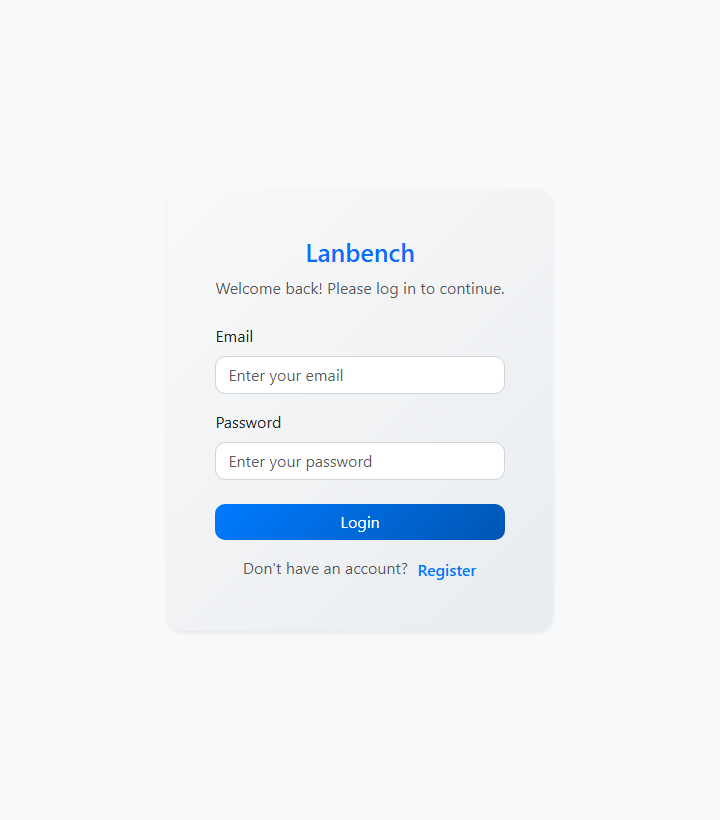
\includegraphics[width=0.78\linewidth]{include/figuras/f-ui-01.png}
	\caption{Pantalla de inicio de sesión de \texttt{lanbench}.}
	\label{fig:ui-login}
\end{figure}

\begin{figure}[ht]
	\centering
	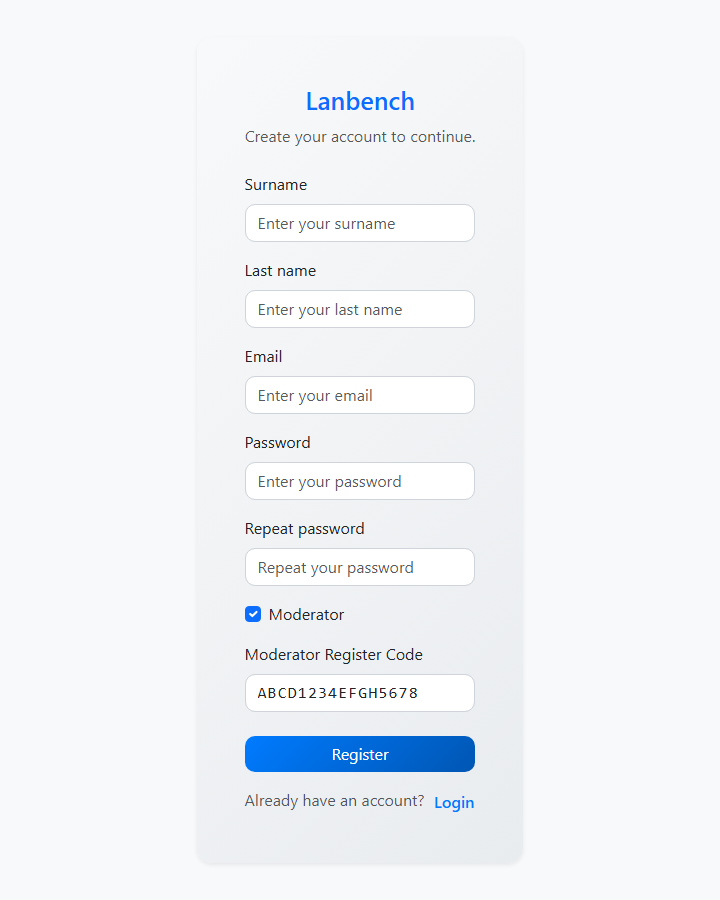
\includegraphics[width=0.78\linewidth]{include/figuras/f-ui-02.png}
	\caption{Pantalla de registro, con el campo opcional de código de
		moderador.}
	\label{fig:ui-register}
\end{figure}

\subsection{Navegación general}

Tras iniciar sesión, una barra de herramientas superior ofrece el acceso a las
áreas principales:

\begin{itemize}
	\item \textbf{Datasets} (\texttt{/datasets}): listado de conjuntos de datos
	      disponibles.
	\item \textbf{Revisión} (\texttt{/reviewer}): cola de revisión de anotaciones.
	\item \textbf{Mis estadísticas} (\texttt{/my-stats}): progreso personal del usuario.
	\item \textbf{Cerrar sesión}: finaliza la sesión activa.
\end{itemize}

\section{Listado y visualización de datasets}

El listado de \textit{datasets} muestra, para cada conjunto, su nombre, su
descripción breve y su estado de progreso. Al seleccionar uno se accede al
\textbf{visualizador del \textit{dataset}} (\texttt{/datasets/:id}), que
organiza la información en varias pestañas:

\begin{itemize}
	\item \textbf{Original}: presenta las tripletas y las referencias tal como se
	      importaron.
	\item \textbf{Extendido}: muestra el contenido con las anotaciones en español
	      incorporadas.
	\item \textbf{Solo lectura}: ofrece una vista no editable del material.
	\item \textbf{Visualización del XML}: permite inspeccionar el XML del
	      \textit{dataset} y descargarlo.
\end{itemize}

Desde esta vista, el usuario con acceso puede \textbf{descargar el XML
	original} para inspeccionarlo o reutilizarlo y, cuando el \textit{dataset} está
íntegramente completado, \textbf{descargar el XML extendido} con las
anotaciones en español ya integradas. Las Figuras~\ref{fig:ui-datasets-list}
y~\ref{fig:ui-dataset-viewer} ilustran, respectivamente, el listado y el
visualizador del \textit{dataset}.

\begin{figure}[ht]
	\centering
	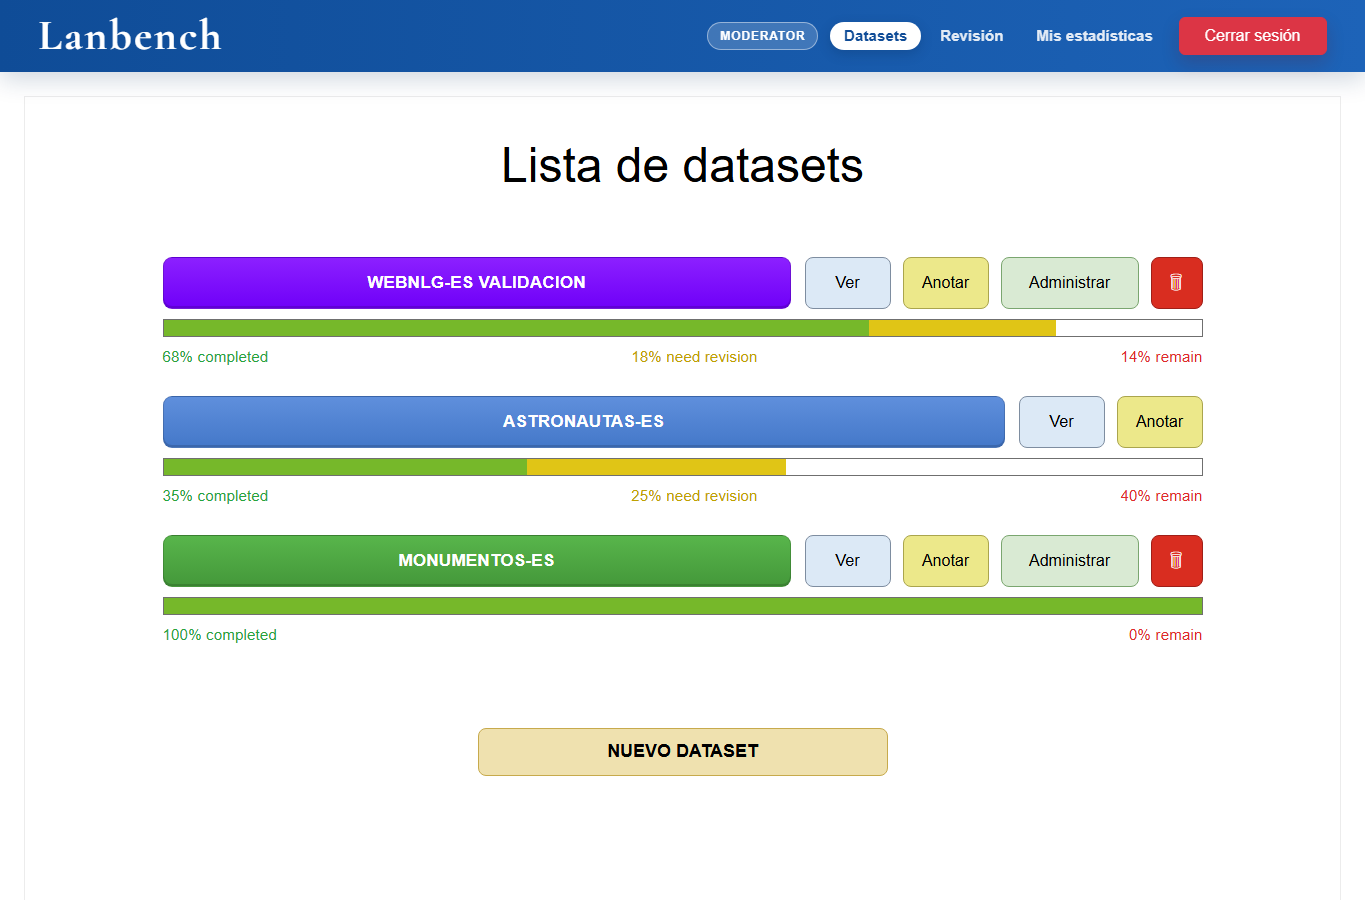
\includegraphics[width=0.92\linewidth]{include/figuras/f-ui-03.png}
	\caption{Listado de \textit{datasets} disponibles.}
	\label{fig:ui-datasets-list}
\end{figure}

\begin{figure}[ht]
	\centering
	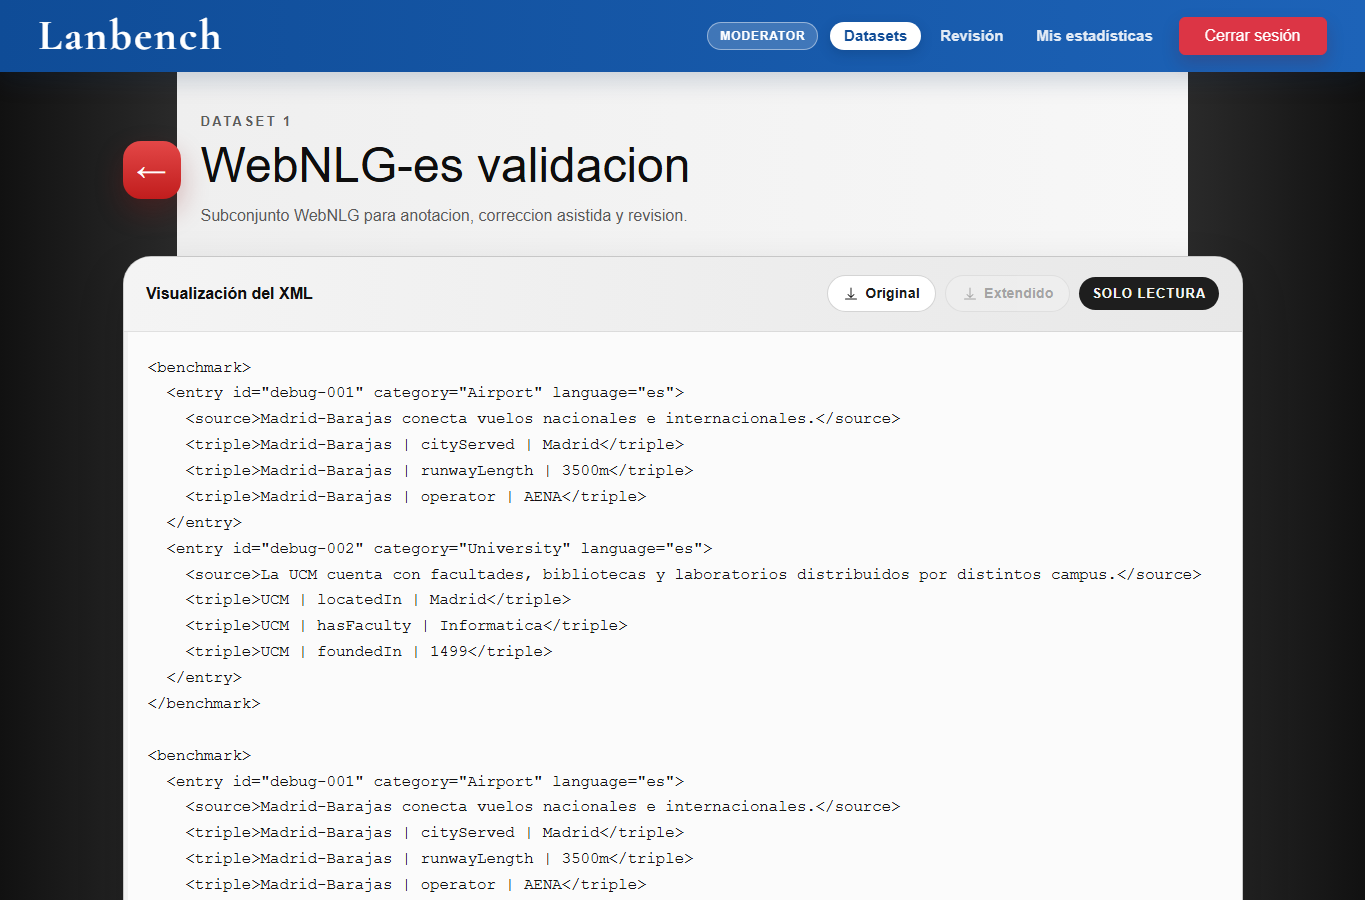
\includegraphics[width=0.92\linewidth]{include/figuras/f-ui-04.png}
	\caption{Visualizador del \textit{dataset} con sus cuatro pestañas
		(Original, Extendido, Solo lectura, XML).}
	\label{fig:ui-dataset-viewer}
\end{figure}

\section{Anotación}

La pantalla de anotación presenta la tarea \emph{RDF a español} sobre la
sección asignada al usuario. El flujo de trabajo habitual es el siguiente:

\begin{enumerate}
	\item \textbf{Lectura de las tripletas}: el sistema presenta el conjunto de tripletas
	      RDF de la entrada de forma legible, de manera que se comprenda la información
	      que debe verbalizarse.
	\item \textbf{Redacción}: el anotador escribe la sentencia en español. Puede partir
	      directamente de las tripletas o apoyarse en la referencia en inglés, sin perder
	      el foco en la cobertura de todas las tripletas. Cuando el \textit{dataset}
	      opera en modo de generación, puede partir de una propuesta automática y
	      limitarse a corregirla.
	\item \textbf{Validación}: el \textit{panel de validación} comprueba que el texto
	      cubre todas las tripletas y señala posibles incidencias antes de guardar.
	\item \textbf{Alertas automáticas}: al finalizar la anotación, el sistema genera
	      alertas de tipo ortográfico, gramatical y semántico. El anotador puede
	      aceptarlas y aplicar la corrección o, si decide omitir alguna, debe justificar
	      la omisión para que el revisor pueda revalidarla.
	\item \textbf{Guardado y avance}: una vez guardada la anotación se avanza a la
	      siguiente entrada. La interfaz informa cuando una \textbf{sección} o el
	      \textbf{\textit{dataset}} completo han quedado finalizados.
\end{enumerate}

\begin{figure}[ht]
	\centering
	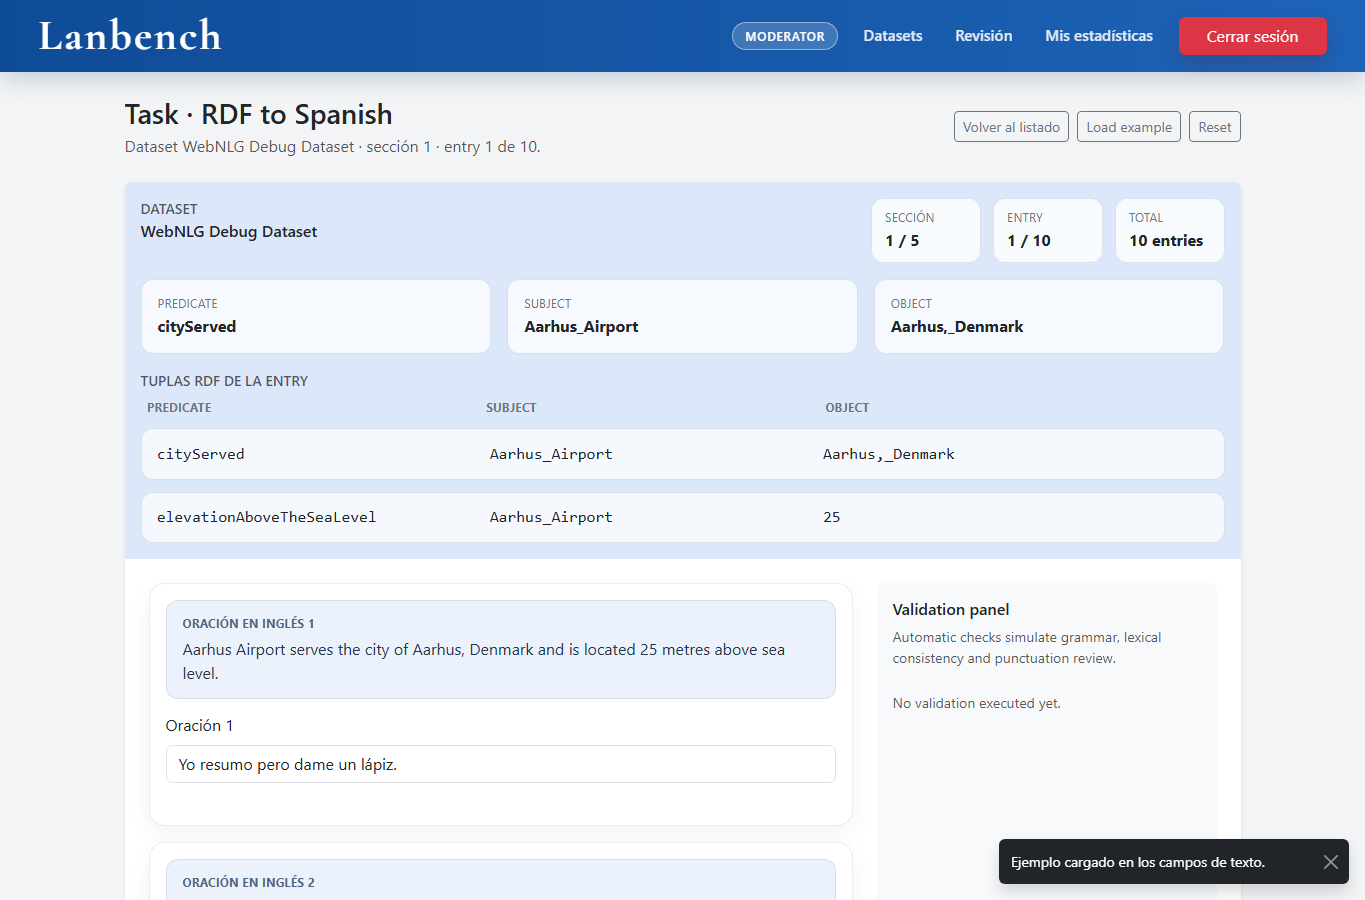
\includegraphics[width=0.92\linewidth]{include/figuras/f-ui-05.png}
	\caption{Pantalla de anotación con el panel de validación y las alertas
		automáticas.}
	\label{fig:ui-annotation}
\end{figure}

\section{Revisión}

La pantalla de revisión (\texttt{/reviewer}) presenta, para cada entrada de la
cola, sus \textbf{frases anotadas} y los \textbf{criterios de calidad} con los
que evaluarlas. El asistente funciona del siguiente modo:

\begin{itemize}
	\item La evaluación se realiza \textbf{frase a frase}. Los cinco criterios de frase
	      ---naturalidad, fluidez, adecuación, completitud y cobertura--- se aplican de forma
	      secuencial: hasta que el criterio actual no se decide, el siguiente permanece
	      bloqueado. Es posible retroceder y reescribir una decisión anterior dentro de
	      la misma frase.
	\item Existe un criterio adicional, la \textbf{diversidad}, que se decide una única
	      vez para el conjunto de la entrada y solo cuando esta contiene más de una
	      frase.
	\item La decisión es \textbf{binaria}. Una decisión negativa exige introducir un
	      motivo (de hasta 280 caracteres) y, en los criterios de frase, una corrección
	      obligatoria del texto que debe diferir del original.
	\item El revisor \textbf{no puede revisar sus propias anotaciones}: la cola excluye
	      automáticamente las entradas anotadas por el propio usuario.
\end{itemize}

\begin{figure}[ht]
	\centering
	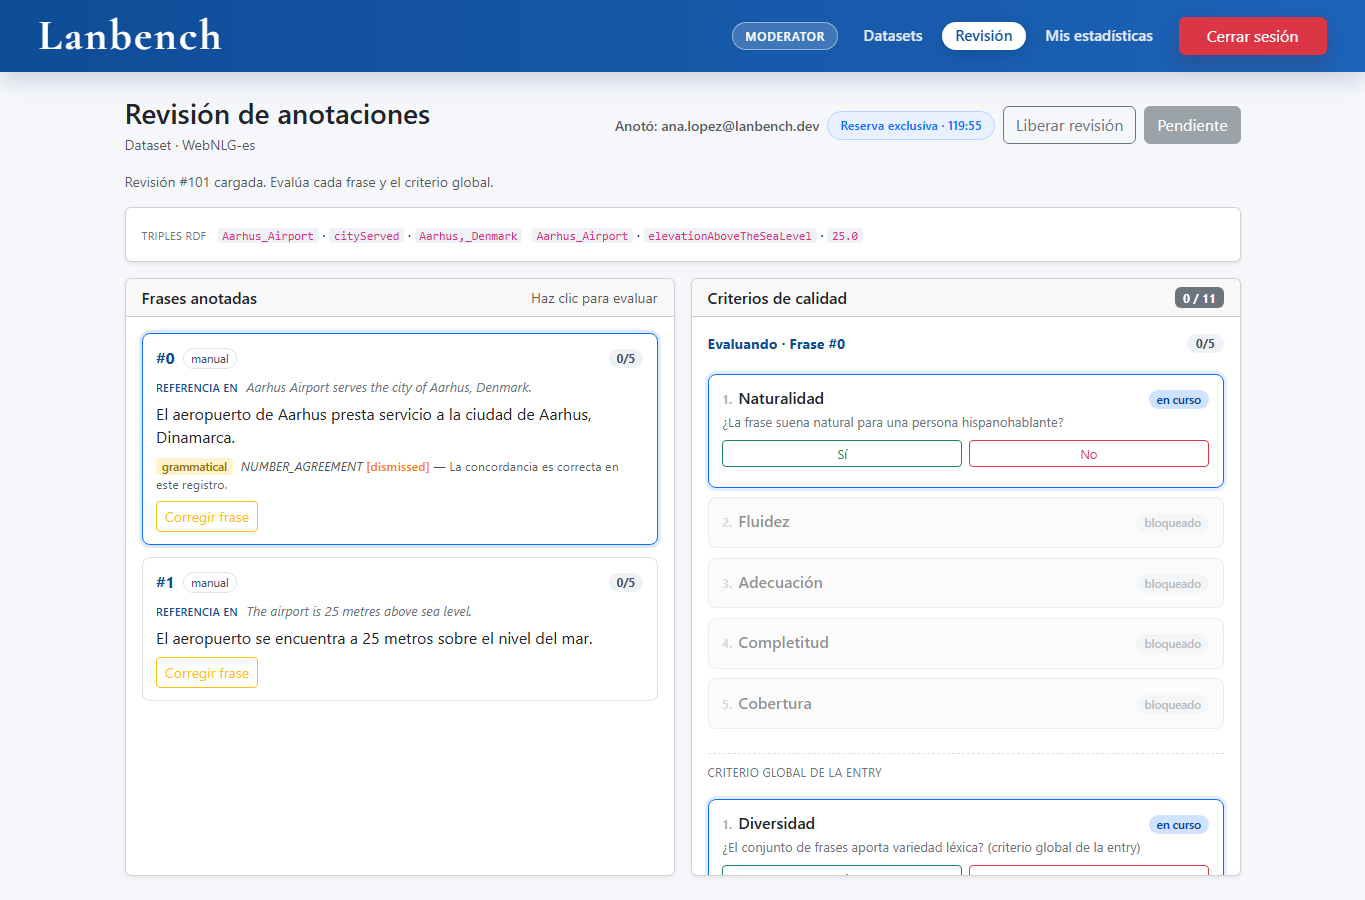
\includegraphics[width=0.92\linewidth]{include/figuras/f-ui-06.png}
	\caption{Pantalla de revisión con el asistente secuencial por criterio.}
	\label{fig:ui-review}
\end{figure}

\section{Estadísticas personales}

La página \emph{Mis estadísticas} (\texttt{/my-stats}) resume el progreso del
usuario \textbf{por \textit{dataset}}. El anotador consulta, entre otros datos,
el número de anotaciones realizadas y los errores subsanados en revisión, lo
que le permite evitar reincidir en ellos; el revisor consulta el número de
revisiones cerradas y el tiempo medio por revisión. La
Figura~\ref{fig:ui-my-stats} ofrece una captura de la pantalla.

\begin{figure}[ht]
	\centering
	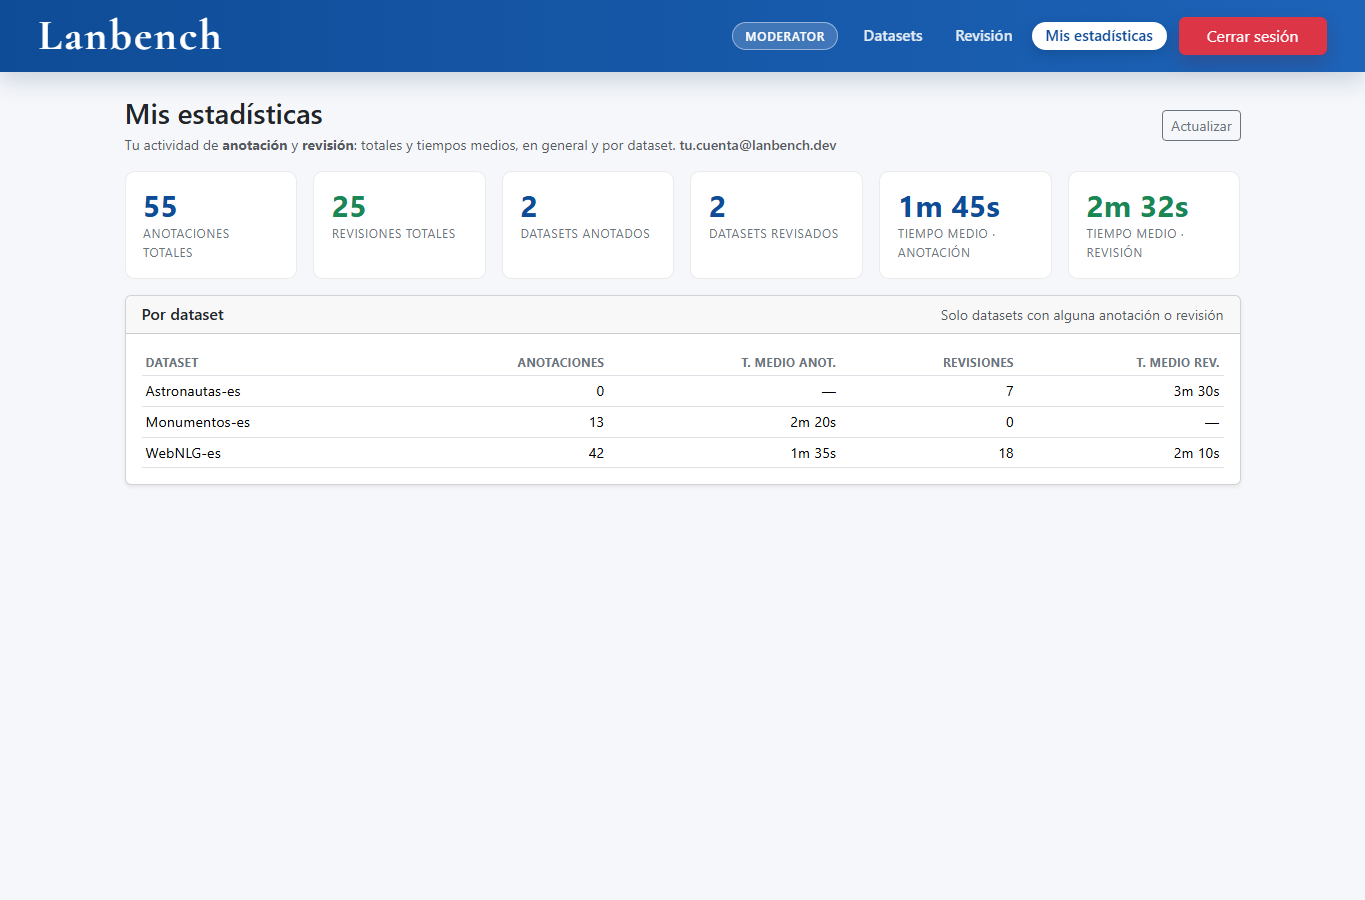
\includegraphics[width=0.92\linewidth]{include/figuras/f-ui-07.png}
	\caption{Pantalla de estadísticas personales del usuario.}
	\label{fig:ui-my-stats}
\end{figure}

\section{Administración del dataset}

Los usuarios con rol de administración sobre un \textit{dataset} disponen de
una página de \textbf{administración} con varias áreas:

\begin{itemize}
	\item \textbf{Creación y opciones}: al crear un \textit{dataset} se sube el fichero
	      RDF y se definen su nombre (con el nombre del fichero como valor por defecto),
	      una descripción breve opcional y las opciones declarativas \emph{tamaño de
		      sección}, \emph{uso de LLM}, \emph{revisión} y \emph{revisiones adicionales
		      tras corrección}. El nombre puede modificarse después, manteniendo su unicidad
	      por propietario.
	\item \textbf{Credenciales de IA}: el administrador del \textit{dataset} registra,
	      activa y comprueba sus propias claves de proveedor (compatibles con OpenAI,
	      Groq, Google AI Studio y Anthropic). Las claves se almacenan cifradas y nunca
	      se devuelven al cliente en claro; el modelo puede elegirse del catálogo público
	      del proveedor, con introducción manual como respaldo.
	\item \textbf{Anotación automática asistida}: en un \textit{dataset} en modo de
	      generación, el administrador puede lanzar la anotación automática, que bloquea
	      un número de secciones y las procesa en segundo plano, con posibilidad de
	      reintentar o cancelar tras un fallo del proveedor.
	\item \textbf{Estadísticas}: el administrador consulta las estadísticas por usuario y
	      un promedio general ponderado de los tiempos de anotación y revisión, junto con
	      la cobertura y los errores subsanados en cada fase, así como las descargas de
	      los avances del \textit{dataset}.
\end{itemize}

\begin{figure}[ht]
	\centering
	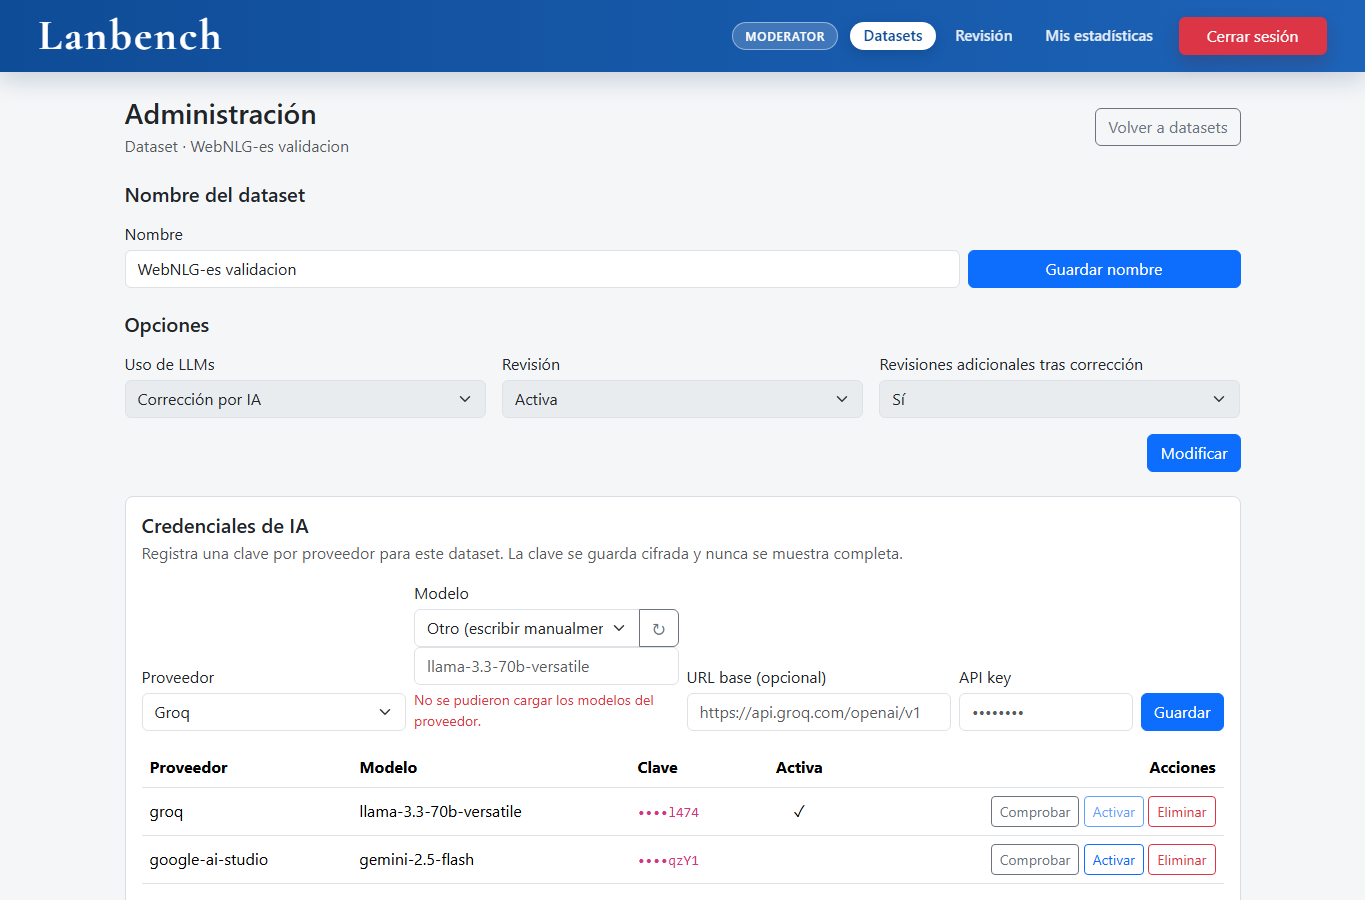
\includegraphics[width=0.92\linewidth]{include/figuras/f-ui-08.png}
	\caption{Pantalla de administración del \textit{dataset}: creación,
		credenciales LLM, lanzamiento de anotación automática y estadísticas.}
	\label{fig:ui-admin-dataset}
\end{figure}

\chapter{Catálogo completo de códigos de validación}

Este anexo reproduce el catálogo declarado en
\texttt{constants/validation-codes.js}, organizado por severidad y categoría.
Los códigos constituyen el lenguaje común entre el componente determinista, el
componente LLM y la interfaz de usuario. La severidad se asigna de forma fija
con independencia del proveedor, de modo que el sistema visual sea estable
incluso ante un cambio de modelo.

\begin{longtable}{|p{0.26\linewidth}|p{0.13\linewidth}|p{0.18\linewidth}|p{0.36\linewidth}|}
	\hline
	\textbf{Código}                  & \textbf{Severidad} & \textbf{Categoría} & \textbf{Mensaje base}                                         \\
	\hline
	\endhead
	\texttt{ok}                      & ok                 & none               & Sin errores detectados.                                       \\ \hline
	\texttt{spelling\_error}         & error              & orthography        & Falta ortográfica.                                            \\ \hline
	\texttt{grammar\_error}          & error              & grammar            & Error sintáctico.                                             \\ \hline
	\texttt{semantic\_mismatch}      & error              & semantic           & La traducción no refleja el significado del triple.           \\ \hline
	\texttt{rdf\_error}              & error              & coverage           & La verbalización del triple es incorrecta o incompleta.       \\ \hline
	\texttt{language\_not\_spanish}  & error              & grammar            & La oración no está escrita en español.                        \\ \hline
	\texttt{mixed\_language}         & error              & grammar            & La oración mezcla español con otro idioma.                    \\ \hline
	\texttt{incomplete\_sentence}    & error              & coverage           & La oración no verbaliza el predicado del triple.              \\ \hline
	\texttt{inverted\_relation}      & error              & semantic           & La relación RDF se expresa de forma invertida.                \\ \hline
	\texttt{missing\_triple}         & error              & coverage           & La oración omite uno o más triples requeridos.                \\ \hline
	\texttt{relation\_missing}       & error              & coverage           & La oración no verbaliza la relación del triple.               \\ \hline
	\texttt{relation\_inverted}      & error              & semantic           & La relación se expresa de forma invertida respecto al triple. \\ \hline
	\texttt{imprecise\_entity\_name} & warning            & semantic           & Nombre de entidad impreciso respecto al triple.               \\ \hline
	\texttt{vague\_translation}      & warning            & semantic           & Traducción vaga o poco precisa.                               \\ \hline
	\texttt{accent\_error}           & warning            & orthography        & Acento incorrecto.                                            \\ \hline
	\texttt{missing\_comma}          & warning            & grammar            & Falta coma en la oración.                                     \\ \hline
	\texttt{punctuation\_missing}    & warning            & grammar            & Signo de puntuación ausente o incorrecto.                     \\ \hline
	\texttt{unnatural\_expression}   & warning            & grammar            & Expresión no natural en español.                              \\ \hline
	\texttt{repeated\_sentence}      & duplicate          & diversity          & Oración repetida: existe una idéntica o muy similar.          \\ \hline
\end{longtable}

La severidad \textit{duplicate} se reserva para una única regla
(\texttt{repeated\_sentence}) que se determina en una pasada determinista
comparativa entre las frases de la misma entrada y, por tanto, no participa en
el catálogo entregado al LLM.

\chapter{Instrucciones de sistema (\textit{system prompts}) utilizadas con los LLM}

La reproducibilidad de los experimentos descritos en el capítulo
correspondiente exige documentar las instrucciones exactas suministradas al
modelo de lenguaje. A continuación se reproducen los \textit{system prompts}
empleados por el \textit{pipeline} de corrección en sus dos modalidades, en su
forma vigente al cierre del experimento descrito.

\section{\textit{Prompt} de comprobación individual}

\begin{verbatim}
Eres un revisor experto de oraciones en espanol para un benchmark RDF.
Debes revisar ortografia, gramatica, puntuacion y adecuacion semantica
respecto a los triples y la frase inglesa de referencia.
Responde SOLO en JSON con este formato exacto:
{"valid":boolean, "reason":string|null, "suggestion":string|null}
Si la oracion es correcta, usa
{"valid":true, "reason":null, "suggestion":null}.
Si no es correcta, explica el problema en "reason" y devuelve en
"suggestion" una version corregida en espanol.
\end{verbatim}

\section{\textit{Prompt} de comprobación por lotes}

El \textit{prompt} de la modalidad \texttt{checkBatch} introduce restricciones
adicionales orientadas a estabilizar la salida ante candidatas múltiples y a
desambiguar los códigos ortográficos:

\begin{verbatim}
Eres un revisor estricto de traducciones espanolas para un benchmark RDF.
Recibiras una entrada JSON con triples, referencias inglesas y candidatas
espanolas. Valida CADA candidata de forma independiente.
sentenceIndex identifica la candidata, no el triple. No inventes indices
de triple.
Si una referencia tiene english=null, recibiras ademas rdfSchematic con
la tripleta cruda; tratala SOLO como recordatorio del triple, NUNCA como
traduccion a comparar literalmente.
Cada candidata debe ser una oracion espanola completa, no un fragmento.
Marca error si la candidata esta en ingles, mezcla idiomas, omite la
relacion del triple, cambia entidad/fecha/numero, invierte la relacion o
solo menciona entidades sin verbalizar el predicado.
Distingue dos casos ortograficos:
  (a) ausencia de tildes/acentos => accent_error (severity warning);
  (b) errores de letras (kapital, hamburgesa) => spelling_error
       (severity error).
Codigos permitidos: <catalogo sin "ok" y sin "repeated_sentence">.
El campo "code" debe ser EXACTAMENTE uno de los codigos permitidos. El
campo "explanation" debe contener SOLO la parte variable del problema.
\end{verbatim}

La omisión deliberada de los códigos \texttt{ok} y \texttt{repeated\_sentence}
del listado entregado al LLM es funcional: el primero se infiere por ausencia
de incidencia, y el segundo se determina en una pasada determinista
comparativa, no por juicio del modelo.

\chapter{Incidencias resueltas durante la integración con proveedores LLM}
\label{anx:incidencias}

Este anexo documenta las incidencias técnicas detectadas durante la preparación
del entorno experimental, así como las correcciones aplicadas para su
resolución. Su inclusión persigue el doble objetivo de garantizar la
reproducibilidad del experimento y de dejar trazabilidad de las decisiones de
ingeniería tomadas.

\section{Cliente compatible con la API de OpenAI: rol \texttt{system} vacío}

La ejecución del experimento requirió como paso previo la resolución de una
incidencia detectada en la comprobación de credenciales de Groq. El cliente
genérico construía el campo \texttt{messages} del cuerpo de la petición
incluyendo siempre un mensaje de rol \texttt{system}, incluso cuando el
\textit{system prompt} no se había proporcionado. Bajo esta condición, el
\textit{endpoint} de Groq devolvía un error de validación:

\begin{verbatim}
groq respondió con 400: {"error":{"message":"'messages.0' : for
'role:system' the following must be satisfied
[('messages.0.content' : property 'content' is missing)]"}}
\end{verbatim}

La corrección consistió en construir defensivamente el \textit{array} de
mensajes, incluyendo el rol \texttt{system} únicamente cuando se proporciona un
\textit{prompt} no vacío, replicando así el comportamiento del cliente nativo
de Anthropic. La regresión queda cubierta por el \textit{spec}
\texttt{tests/unit/ollama/openai-compatible-client.test.js}, que verifica que
el mensaje de sistema se omite cuando no se especifica.

\chapter{Licenciamiento y datos personales}

\section{Licencia del corpus}

El corpus WebNLG se distribuye bajo licencia Creative Commons
Attribution-ShareAlike, lo que permite la reutilización siempre que se mantenga
la atribución y se preserve la misma licencia para los derivados. La extensión
al español propuesta en este trabajo se publica, en consecuencia, bajo idéntica
licencia para garantizar compatibilidad con el corpus madre y con sus ediciones
bilingües previas.

\section{Datos personales y RGPD}

En relación con los datos personales, el sistema solamente almacena la
información mínima necesaria para identificar al usuario en el flujo de
\textit{crowdsourcing}: correo electrónico, nombre y apellidos, huella derivada
de la contraseña y rol. No se conservan datos sensibles más allá de las
sesiones activas y de los registros de actividad documentados en el capítulo de
la aplicación. Esta política se ajusta al principio de minimización del
Reglamento General de Protección de Datos~\cite{GDPR2016} y al criterio
operativo descrito en ~\ref{sec:etica-crowdsourcing}.
